\documentclass[12pt, a4paper]{article}

% ============================================================
% Packages
% ============================================================
\usepackage[margin=1in]{geometry}
\usepackage{titlesec}
\usepackage{enumitem}
\usepackage{hyperref}
\usepackage{graphicx}
\usepackage{booktabs}
\usepackage{tabularx}
\usepackage{xcolor}
\usepackage{fancyhdr}
\usepackage{amsmath}
\usepackage{parskip}
\usepackage{multicol}
\usepackage{tikz}
\usepackage[backend=biber, style=ieee, sorting=nyt]{biblatex}

% ============================================================
% Colors & Styling
% ============================================================
\definecolor{metroBlue}{RGB}{0, 70, 140}
\definecolor{darkGray}{RGB}{50, 50, 50}

\hypersetup{
    colorlinks=true,
    linkcolor=metroBlue,
    urlcolor=metroBlue,
    citecolor=metroBlue
}

\titleformat{\section}{\large\bfseries\color{metroBlue}}{\thesection.}{0.5em}{}[\vspace{-0.5em}\rule{\textwidth}{0.4pt}]
\titleformat{\subsection}{\normalsize\bfseries\color{darkGray}}{\thesubsection}{0.5em}{}

% ============================================================
% Header / Footer
% ============================================================
\pagestyle{fancy}
\fancyhf{}
\rhead{\small\textcolor{gray}{B.Sc. Thesis Proposal}}
\lhead{\small\textcolor{gray}{AEGIS BOT SHIELD}}
\rfoot{\small\textcolor{gray}{Page \thepage}}

% ============================================================
% Title Page
% ============================================================
\begin{document}

\begin{titlepage}
\centering

\vspace*{1cm}

{\Large\textbf{Metropolitan University, Sylhet}}\\[0.3cm]
{\large Department of Computer Science \& Engineering}\\[1.5cm]

\rule{\textwidth}{1.5pt}\\[0.6cm]
{\LARGE\bfseries\color{metroBlue} B.Sc. Thesis Proposal}\\[0.3cm]
\rule{\textwidth}{1.5pt}\\[1.5cm]

{\Large\bfseries AEGIS BOT SHIELD: A Multi-Layered Intelligent\\[0.2cm]
Bot Detection and Defense Framework Using\\[0.2cm]
Ensemble Machine Learning and\\[0.2cm]
Behavioral Biometric Analysis}\\[2cm]

\begin{tabular}{rl}
\textbf{Submitted by:} & Dipro Debnath \\
\textbf{Student ID:} & [Your Student ID] \\
\textbf{Program:} & B.Sc. in Computer Science \& Engineering \\
\textbf{Semester:} & Fall 2026 (Final Semester) \\
\textbf{Email:} & [your.email@metrouni.edu.bd] \\[0.5cm]
\textbf{Supervisor:} & Rishad Amin Pulok \\
\textbf{Designation:} & Lecturer, Dept. of CSE \\
\textbf{Email:} & pulok@metrouni.edu.bd \\
\end{tabular}

\vfill

{\large\textbf{Date of Submission:} \today}

\end{titlepage}

% ============================================================
% Table of Contents
% ============================================================
\tableofcontents
\newpage

% ============================================================
% 1. Introduction
% ============================================================
\section{Introduction}

The rapid growth of web-based applications and services has been accompanied by an equally rapid evolution of automated bot attacks. According to the Imperva Bad Bot Report 2025, automated bot traffic now accounts for approximately 32.4\% of all internet traffic, with malicious bots constituting a significant portion~\cite{imperva2025}. These bots perform a wide range of harmful activities, including credential stuffing, web scraping, distributed denial-of-service (DDoS) attacks, account takeover (ATO), and fraudulent transactions~\cite{owasp_oat}.

Traditional bot detection methods, such as CAPTCHAs and static rule-based systems, have become increasingly inadequate. Modern bots leverage headless browsers (e.g., Puppeteer, Playwright), residential proxy networks, and even large language models (LLMs) to mimic legitimate human behavior~\cite{jonker2019}. The arms race between bot operators and defense systems necessitates a paradigm shift toward \textit{intelligent, multi-layered defense architectures} that combine behavioral biometrics, network intelligence, and machine learning.

This thesis proposes \textbf{AEGIS BOT SHIELD}, a comprehensive, open-source bot detection and defense framework that integrates five distinct defense layers with an ensemble machine learning pipeline. The system collects over 50 behavioral features from client-side interactions (mouse dynamics, keystroke timing, scroll patterns) and combines them with server-side signals (IP intelligence, TLS fingerprinting, HTTP/2 analysis) to classify traffic as human or bot with high accuracy.

The name \textit{AEGIS} derives from Greek mythology—the protective shield of Zeus—symbolizing robust, multi-layered protection for modern web applications.

% ============================================================
% 2. Problem Statement
% ============================================================
\section{Problem Statement}

Despite significant advances in cybersecurity, automated bot attacks continue to inflict substantial damage on web services globally. The key challenges that motivate this research include:

\begin{enumerate}[leftmargin=*, label=\textbf{C\arabic*.}]
    \item \textbf{Evolving Bot Sophistication:} Modern bots employ anti-detection techniques such as residential proxy routing, browser fingerprint spoofing, and human-like behavioral emulation, rendering traditional detection methods ineffective~\cite{iliou2021}.

    \item \textbf{CAPTCHA Degradation:} CAPTCHAs create user friction and are increasingly solvable by AI systems. Google's reCAPTCHA v3 operates silently but remains a black-box solution with no transparency into its decision-making process~\cite{akrout2019}.

    \item \textbf{Single-Signal Limitations:} Existing research often focuses on individual detection signals (e.g., mouse dynamics alone or IP reputation alone). No comprehensive open-source framework combines \textit{all} major detection modalities into a unified decision engine.

    \item \textbf{Lack of Contextual Research:} There is limited research on bot attack patterns in the context of South Asian web services, particularly in Bangladesh where e-commerce and digital services are rapidly expanding.

    \item \textbf{Residential Proxy Blind Spot:} Traditional IP-based detection fails against residential proxy networks (e.g., Bright Data, Oxylabs) that route bot traffic through legitimate residential IPs, making IP reputation alone unreliable~\cite{mi2019}.
\end{enumerate}

\subsection{Research Questions}

This thesis seeks to answer the following research questions:

\begin{enumerate}[leftmargin=*, label=\textbf{RQ\arabic*.}]
    \item How effectively can an ensemble of machine learning models (XGBoost, Random Forest, Logistic Regression) distinguish between human and bot traffic using multi-modal behavioral features?

    \item Which behavioral signal categories (mouse dynamics, keystroke timing, scroll patterns, network fingerprints) contribute most significantly to bot detection accuracy?

    \item Can a multi-layered defense architecture achieve higher detection rates than single-layer approaches while maintaining low false-positive rates ($<$2\%)?

    \item How resilient is the proposed system against sophisticated evasion techniques, including residential proxy routing and headless browser automation?
\end{enumerate}

% ============================================================
% 3. Research Objectives
% ============================================================
\section{Research Objectives}

\subsection{Primary Objectives}

\begin{enumerate}[leftmargin=*, label=\textbf{O\arabic*.}]
    \item \textbf{Design and implement} a multi-layered bot defense framework (AEGIS BOT SHIELD) integrating five defense layers: network analysis, protocol fingerprinting, behavioral biometrics, machine learning, and active challenges.

    \item \textbf{Develop an ensemble ML pipeline} combining XGBoost Gradient Boosted Trees, Random Forest, and Logistic Regression with a meta-learner for stacked generalization.

    \item \textbf{Extract and evaluate 50+ behavioral features} across seven categories (mouse, keyboard, scroll, touch, session, network, fingerprint) and conduct a category-wise ablation study.

    \item \textbf{Evaluate the system} using standard metrics (Accuracy, Precision, Recall, F1-Score, AUC-ROC) with 5-fold stratified cross-validation.

    \item \textbf{Deploy and test} the framework on a real web application to validate detection performance with live traffic data.
\end{enumerate}

\subsection{Secondary Objectives}

\begin{itemize}[leftmargin=*]
    \item Implement novel residential proxy detection using latency-distance analysis, subnet velocity tracking, and MSS/MTU tunnel detection.
    \item Integrate AI/LLM-targeted honeypot traps as a novel detection technique.
    \item Publish findings as a conference paper at a recognized venue (e.g., IEEE ICCIT, ECCE, or ICIEV).
\end{itemize}

% ============================================================
% 4. Literature Review (Summary)
% ============================================================
\section{Literature Review}

\subsection{Mouse Dynamics for Bot Detection}

Ahmed and Traore~\cite{ahmed2007} pioneered the use of mouse dynamics for user authentication, demonstrating that features such as movement velocity, acceleration, curvature, and click precision can distinguish individual users. Subsequent work by Shen et al.~\cite{shen2013} showed that mouse movement features achieve 95\%+ accuracy in user verification tasks. The Balabit Mouse Dynamics Challenge dataset~\cite{balabit2016} has become a benchmark for mouse-based behavioral analysis.

\subsection{Keystroke Dynamics}

Monrose and Rubin~\cite{monrose2000} established that keystroke timing patterns (dwell time, flight time) are distinctive biometric identifiers. Recent work has applied deep learning to keystroke dynamics with promising results for continuous authentication~\cite{lu2020}.

\subsection{Bot Detection Using Machine Learning}

Iliou et al.~\cite{iliou2021} conducted a comprehensive survey of bot detection techniques, categorizing approaches into behavioral, challenge-based, and fingerprint-based methods. Jonker et al.~\cite{jonker2019} demonstrated that combining multiple detection signals significantly improves accuracy over single-signal approaches.

\subsection{TLS and Network Fingerprinting}

The JA3 TLS fingerprinting technique~\cite{ja3_2017} enabled passive identification of client applications based on TLS Client Hello parameters. The newer JA4+ suite~\cite{ja4_2024} extends this to include HTTP, TCP, and X.509 certificate fingerprints, providing higher granularity.

\subsection{Residential Proxy Detection}

Mi et al.~\cite{mi2019} analyzed the ecosystem of residential proxy services, finding that millions of residential IPs are used to mask bot traffic. Detection of residential proxies requires multi-signal analysis combining latency measurements, ASN classification, and traffic pattern analysis.

\subsection{Research Gap}

While individual techniques have been well-studied, \textbf{no existing open-source framework} combines all major detection modalities (behavioral biometrics, network intelligence, device fingerprinting, ML classification, and active challenges) into a unified, production-ready system. Furthermore, there is \textbf{no published research} evaluating such a multi-layered system specifically in the context of South Asian web services.

% ============================================================
% 5. Proposed Methodology
% ============================================================
\section{Proposed Methodology}

\subsection{System Architecture}

AEGIS BOT SHIELD employs a five-layer defense architecture, as illustrated in Figure~\ref{fig:arch}.

\begin{figure}[h]
\centering
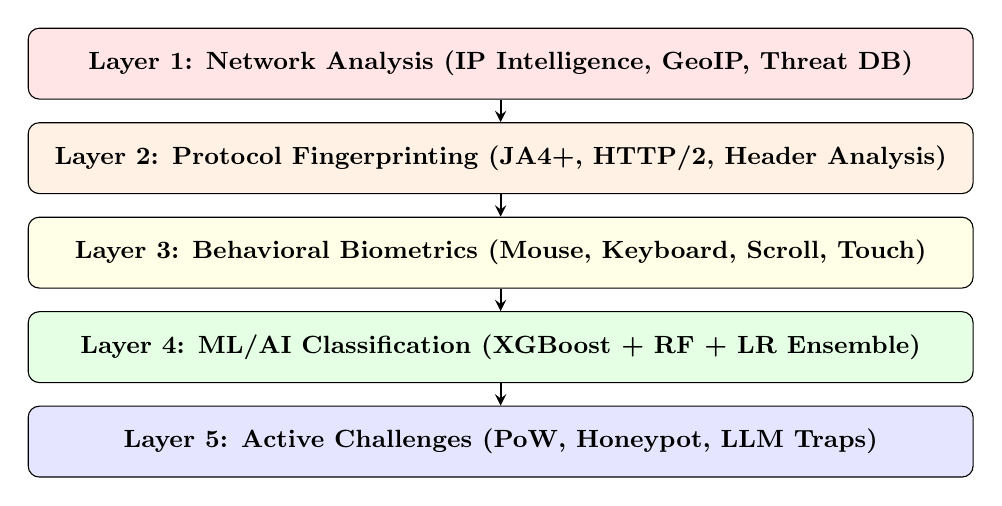
\begin{tikzpicture}[
    layer/.style={draw, rounded corners, minimum width=12cm, minimum height=0.9cm, font=\small\bfseries},
    arrow/.style={->, thick, >=stealth}
]
    \node[layer, fill=red!10] (l1) at (0, 4.5) {Layer 1: Network Analysis (IP Intelligence, GeoIP, Threat DB)};
    \node[layer, fill=orange!10] (l2) at (0, 3.3) {Layer 2: Protocol Fingerprinting (JA4+, HTTP/2, Header Analysis)};
    \node[layer, fill=yellow!10] (l3) at (0, 2.1) {Layer 3: Behavioral Biometrics (Mouse, Keyboard, Scroll, Touch)};
    \node[layer, fill=green!10] (l4) at (0, 0.9) {Layer 4: ML/AI Classification (XGBoost + RF + LR Ensemble)};
    \node[layer, fill=blue!10] (l5) at (0, -0.3) {Layer 5: Active Challenges (PoW, Honeypot, LLM Traps)};

    \draw[arrow] (l1) -- (l2);
    \draw[arrow] (l2) -- (l3);
    \draw[arrow] (l3) -- (l4);
    \draw[arrow] (l4) -- (l5);
\end{tikzpicture}
\caption{AEGIS BOT SHIELD: Five-Layer Defense Architecture}
\label{fig:arch}
\end{figure}

\subsection{Feature Extraction}

The system extracts 50 features across seven categories, as summarized in Table~\ref{tab:features}.

\begin{table}[h]
\centering
\caption{Feature Categories and Key Features}
\label{tab:features}
\small
\begin{tabularx}{\textwidth}{l c X}
\toprule
\textbf{Category} & \textbf{Count} & \textbf{Key Features} \\
\midrule
Mouse Dynamics & 15 & Velocity (mean, std), acceleration, jerk, curvature, straightness index, Fitts' Law $R^2$, micro-tremor frequency, click precision \\
Keyboard Dynamics & 10 & Dwell time, flight time, typing speed, cadence entropy, correction ratio \\
Scroll Behavior & 5 & Velocity, direction changes, depth, momentum ratio \\
Touch Behavior & 5 & Pressure, radius, swipe velocity, tap count \\
Session Patterns & 5 & Duration, request count, unique paths, inter-request timing \\
Network Signals & 5 & VPN/Tor/datacenter flags, residential proxy, IP reputation \\
Device Fingerprint & 5 & WebGL, canvas, plugin count, headless detection confidence \\
\midrule
\textbf{Total} & \textbf{50} & \\
\bottomrule
\end{tabularx}
\end{table}

\subsection{Machine Learning Pipeline}

\subsubsection{Ensemble Architecture}

The classification pipeline employs a \textit{stacked generalization} approach:

\begin{enumerate}[leftmargin=*]
    \item \textbf{Base Learners:}
    \begin{itemize}
        \item XGBoost Gradient Boosted Trees (200 estimators, max\_depth=6)
        \item Random Forest (200 estimators, max\_depth=10)
        \item Logistic Regression (L2 regularization, as interpretable baseline)
    \end{itemize}
    \item \textbf{Meta-Learner:} Logistic Regression trained on stacked predictions of base learners.
    \item \textbf{Anomaly Detection:} Isolation Forest + Local Outlier Factor ensemble for zero-day bot detection (unsupervised component).
\end{enumerate}

\subsubsection{Evaluation Methodology}

\begin{itemize}[leftmargin=*]
    \item \textbf{Data Split:} 70\% training / 15\% validation / 15\% test (stratified)
    \item \textbf{Cross-Validation:} 5-fold stratified K-fold
    \item \textbf{Metrics:} Accuracy, Precision, Recall, F1-Score, AUC-ROC
    \item \textbf{Ablation Study:} Remove each feature category and measure accuracy drop
    \item \textbf{Comparison:} Individual models vs. ensemble vs. baseline (rule-based)
\end{itemize}

\subsection{Data Collection Strategy}

\begin{enumerate}[leftmargin=*]
    \item \textbf{Phase 1 — Synthetic Data (Initial Training):}
    Research-grounded synthetic data generator producing human-like and bot-like behavioral samples with four bot difficulty levels (simple script, headless browser, sophisticated bot, crawler).

    \item \textbf{Phase 2 — Real Data Collection:}
    Deploy AEGIS on a test web application and collect:
    \begin{itemize}
        \item \textit{Human data:} Recruit 30--50 participants to perform browsing tasks (requires Ethics/IRB approval).
        \item \textit{Bot data:} Generate automated traffic using Selenium, Puppeteer, Playwright, curl, and custom Python scripts with varying sophistication levels.
    \end{itemize}

    \item \textbf{Phase 3 — Labeling:}
    All data is automatically labeled based on the collection source (human participants = 0, automation tools = 1).
\end{enumerate}

\textbf{Note:} Ethics/IRB approval will be obtained from the university's ethics committee before collecting data from human participants. All collected data will be anonymized, and participants will provide informed consent.

% ============================================================
% 6. Technology Stack
% ============================================================
\section{Technology Stack}

\begin{table}[h]
\centering
\caption{Technology Stack}
\small
\begin{tabularx}{\textwidth}{l X}
\toprule
\textbf{Component} & \textbf{Technologies} \\
\midrule
Core Detection Engine & TypeScript, Node.js (ESM modules) \\
Client-Side SDK & TypeScript (browser), Canvas API, WebGL, SubtleCrypto \\
Server Middleware & Node.js (Express, Fastify), Python (Django, Flask, FastAPI) \\
ML Engine & Python, scikit-learn, XGBoost, NumPy, Pandas \\
Dashboard & React, TypeScript, Recharts \\
Infrastructure & Docker, GitHub Actions CI/CD, Redis (caching) \\
Cryptography & AES-256-GCM, HMAC-SHA256, Proof-of-Work (SHA-256) \\
\bottomrule
\end{tabularx}
\end{table}

% ============================================================
% 7. Expected Contributions
% ============================================================
\section{Expected Contributions}

\begin{enumerate}[leftmargin=*, label=\textbf{EC\arabic*.}]
    \item \textbf{Multi-Layered Framework:} An open-source, production-ready bot defense framework combining five complementary defense layers—the first of its kind as an integrated SDK.

    \item \textbf{Comprehensive Feature Set:} A curated set of 50 behavioral features with empirical evaluation of each category's contribution through ablation analysis.

    \item \textbf{Ensemble ML Pipeline:} A stacked generalization approach combining XGBoost, Random Forest, and Logistic Regression, benchmarked against individual models.

    \item \textbf{Novel Detection Techniques:}
    \begin{itemize}
        \item Residential proxy detection via latency-distance correlation and MSS/MTU tunnel analysis.
        \item AI/LLM-targeted honeypot traps using prompt injection canaries.
        \item Adaptive rate limiting with statistical attack pattern detection.
    \end{itemize}

    \item \textbf{Reproducible Research:} Fully open-source codebase on GitHub with synthetic data generator enabling reproduction of results.
\end{enumerate}

% ============================================================
% 8. Timeline
% ============================================================
\section{Project Timeline}

\begin{table}[h]
\centering
\caption{Semester Timeline (September -- December 2026)}
\small
\begin{tabularx}{\textwidth}{l l X}
\toprule
\textbf{Period} & \textbf{Phase} & \textbf{Activities} \\
\midrule
Sept 1--30 & Development & System implementation, 30-day feature sprint \\
& & Literature review and related work survey \\[0.3cm]

Oct 1--31 & Deployment \& & Deploy test website with AEGIS integration \\
& Data Prep & Ethics/IRB approval submission \\
& & Prepare data collection instruments \\[0.3cm]

Nov 1--30 & Data Collection & Recruit human participants (30--50 users) \\
& \& Evaluation & Generate bot traffic (multiple sophistication levels) \\
& & Train ML models on real data \\
& & Run ablation study and model comparison \\[0.3cm]

Dec 1--15 & Analysis \& & Statistical analysis of results \\
& Writing & Thesis document drafting \\
& & Conference paper preparation \\[0.3cm]

Dec 16--30 & Finalization & Thesis defense preparation \\
& & Submit conference paper (ICCIT / ECCE deadline) \\
& & Final revisions \\
\bottomrule
\end{tabularx}
\end{table}

% ============================================================
% 9. Current Progress
% ============================================================
\section{Current Progress}

Development of the AEGIS BOT SHIELD framework has already commenced. As of the date of this proposal, the following milestones have been achieved:

\begin{itemize}[leftmargin=*]
    \item \textbf{Complete system architecture} designed with 6 packages (core engine, JS SDK, Node.js server, Python server, ML engine, dashboard).
    \item \textbf{Core detection engine} fully implemented with 13 detection modules ($\sim$3,500 lines of TypeScript).
    \item \textbf{Client-side JS SDK} with behavioral collectors and 17+ headless detection tests.
    \item \textbf{ML engine} with feature extraction (50 features), ensemble classifier, anomaly detector, and synthetic data generator.
    \item \textbf{Server middleware} for Express.js, Fastify, Django, Flask, and FastAPI.
    \item \textbf{React dashboard} with real-time visualization and ML performance metrics.
    \item \textbf{GitHub repository:} \url{https://github.com/dipro20debnath/AEGIS-BOT-SHIELD} (8 commits, 8,500+ lines of code).
\end{itemize}

% ============================================================
% 10. Ethical Considerations
% ============================================================
\section{Ethical Considerations}

\begin{itemize}[leftmargin=*]
    \item \textbf{Informed Consent:} All human participants will sign consent forms before data collection. Participants will be briefed on what data is collected and how it will be used.
    \item \textbf{Data Anonymization:} No personally identifiable information (PII) will be stored. Behavioral data will be anonymized and identified only by random session IDs.
    \item \textbf{Privacy Protection:} The keystroke collector records \textit{timing only} (not actual key values), ensuring user input remains private.
    \item \textbf{IRB Approval:} Ethics/IRB approval will be obtained from the university's ethics committee prior to human data collection.
    \item \textbf{Responsible Disclosure:} All bot detection techniques are designed for defensive purposes only.
\end{itemize}

% ============================================================
% 11. Conclusion
% ============================================================
\section{Conclusion}

This thesis proposes AEGIS BOT SHIELD, a multi-layered intelligent bot detection and defense framework that addresses the growing threat of automated bot attacks through the integration of behavioral biometrics, network intelligence, device fingerprinting, and ensemble machine learning. The framework's five-layer architecture provides defense-in-depth, while the 50-feature ML pipeline enables high-accuracy classification with comprehensive ablation analysis. The open-source nature of the project ensures reproducibility and real-world applicability.

The successful completion of this thesis will contribute a novel, production-ready framework to the cybersecurity community while advancing academic understanding of multi-modal bot detection through rigorous empirical evaluation.

% ============================================================
% References
% ============================================================
\newpage
\section*{References}
\addcontentsline{toc}{section}{References}

\begin{thebibliography}{99}

\bibitem{imperva2025}
Imperva, ``2025 Bad Bot Report,'' Imperva Research Labs, 2025. [Online]. Available: \url{https://www.imperva.com/resources/reports/2025-bad-bot-report/}

\bibitem{owasp_oat}
OWASP, ``Automated Threats to Web Applications,'' OWASP Foundation, 2023. [Online]. Available: \url{https://owasp.org/www-project-automated-threats-to-web-applications/}

\bibitem{ahmed2007}
A. A. E. Ahmed and I. Traore, ``A New Biometric Technology Based on Mouse Dynamics,'' \textit{IEEE Trans. Dependable Secure Comput.}, vol. 4, no. 3, pp. 165--179, Jul. 2007.

\bibitem{shen2013}
C. Shen, Z. Cai, and X. Guan, ``Continuous Authentication for Mouse Dynamics: A Pattern-Growth Approach,'' in \textit{Proc. IEEE/IFIP Int. Conf. Dependable Syst. Netw. (DSN)}, 2013, pp. 1--12.

\bibitem{balabit2016}
Balabit, ``Mouse Dynamics Challenge Dataset,'' 2016. [Online]. Available: \url{https://github.com/balabit/Mouse-Dynamics-Challenge}

\bibitem{monrose2000}
F. Monrose and A. D. Rubin, ``Keystroke Dynamics as a Biometric for Authentication,'' \textit{Future Generation Comput. Syst.}, vol. 16, no. 4, pp. 351--359, 2000.

\bibitem{lu2020}
X. Lu, S. Zhang, and P. Hui, ``Continuous Authentication by Free-Text Keystroke Based on CNN and RNN,'' \textit{Comput. Secur.}, vol. 96, p. 101861, 2020.

\bibitem{iliou2021}
C. Iliou, T. Kostoulas, T. Tsikrika, V. Katos, S. Vrochidis, and I. Kompatsiaris, ``Detection of Advanced Web Bots by Combining Web Logs with Mouse Behavioural Biometrics,'' \textit{Digital Threats: Res. Pract.}, vol. 2, no. 3, pp. 1--26, 2021.

\bibitem{jonker2019}
H. Jonker, B. Krumnow, and G. Vlot, ``Fingerprint Surface-Based Detection of Web Bot Detectors,'' in \textit{Proc. European Symp. Res. Comput. Secur. (ESORICS)}, 2019, pp. 586--605.

\bibitem{akrout2019}
I. Akrout, A. Feriani, and M. Akrout, ``Hacking Google reCAPTCHA v3 Using Reinforcement Learning,'' \textit{arXiv preprint arXiv:1903.01003}, 2019.

\bibitem{ja3_2017}
J. Althouse, J. Atkinson, and J. Atkins, ``JA3 - A Method for Profiling SSL/TLS Clients,'' Salesforce Engineering, 2017. [Online]. Available: \url{https://github.com/salesforce/ja3}

\bibitem{ja4_2024}
J. Althouse, ``JA4+ Network Fingerprinting,'' FoxIO, 2024. [Online]. Available: \url{https://github.com/FoxIO-LLC/ja4}

\bibitem{mi2019}
X. Mi, X. Feng, X. Liao, B. Liu, X. Wang, F. Qian, Z. Li, S. Alrwais, L. Sun, and Y. Liu, ``Resident Evil: Understanding Residential IP Proxy as a Dark Service,'' in \textit{Proc. IEEE Symp. Secur. Privacy (S\&P)}, 2019, pp. 1185--1201.

\bibitem{fitts1954}
P. M. Fitts, ``The Information Capacity of the Human Motor System in Controlling the Amplitude of Movement,'' \textit{J. Exp. Psychol.}, vol. 47, no. 6, pp. 381--391, 1954.

\bibitem{sklearn}
F. Pedregosa et al., ``Scikit-learn: Machine Learning in Python,'' \textit{J. Mach. Learn. Res.}, vol. 12, pp. 2825--2830, 2011.

\bibitem{xgboost}
T. Chen and C. Guestrin, ``XGBoost: A Scalable Tree Boosting System,'' in \textit{Proc. 22nd ACM SIGKDD}, 2016, pp. 785--794.

\end{thebibliography}

% ============================================================
% Signature
% ============================================================
\vspace{2cm}

\noindent
\begin{minipage}[t]{0.45\textwidth}
\centering
\rule{5cm}{0.4pt}\\
\textbf{Dipro Debnath}\\
Student\\
Dept. of CSE\\
Metropolitan University, Sylhet
\end{minipage}
\hfill
\begin{minipage}[t]{0.45\textwidth}
\centering
\rule{5cm}{0.4pt}\\
\textbf{Rishad Amin Pulok}\\
Supervisor (Lecturer)\\
Dept. of CSE\\
Metropolitan University, Sylhet
\end{minipage}

\end{document}
